\section{Unified Foundation Architecture}
\label{sec:architecture}

\subsection{Shared Backbone}

The architecture follows a familiar audio-encoder--adapter--LLM-decoder pattern that has become central to audio-language modeling~\citep{wu2025stepaudio2technicalreport,xu2025qwen3omnitechnicalreport}. A frozen audio encoder converts waveform-derived features into compact acoustic embeddings. A lightweight adaptor maps those embeddings into the hidden space of a large decoder initialized from a text LLM. The decoder then operates over a unified sequence space in which conventional text tokens and newly introduced audio tokens can both appear.

This design is intentionally asymmetric. The encoder is responsible for stable acoustic abstraction, while the decoder carries the burden of semantics, context management, instruction following, and generation. Such asymmetry is not a limitation; it is the systems decision that makes the model family coherent. Once semantics live primarily in the decoder, downstream tasks can share most of the model even when their outputs differ.

Figure~\ref{fig:unified_architecture} summarizes the structural organization used throughout this report. At the center is the shared StepAudio 2.5 foundation model, which supports three model-level specializations: ASR, TTS, and Realtime. These three systems share the same audio-language stack while serving different deployment regimes, making the figure a compact summary of how one foundation is specialized for recognition, synthesis, and live spoken interaction.

% \begin{figure}[tbp]
% \centering
% \resizebox{0.92\linewidth}{!}{%
% \begin{tikzpicture}[
% node distance=7mm and 9mm,
% box/.style={draw, rounded corners, thick, align=center, fill=gray!8, minimum width=3.3cm, minimum height=0.9cm},
% arrow/.style={-Latex, thick}
% ]
% \node[box] (audio) {Audio Encoder};
% \node[box, right=of audio] (adapter) {Adaptor};
% \node[box, right=of adapter] (decoder) {LLM Decoder};
% \node[box, below left=12mm and -7mm of decoder, minimum width=3.2cm] (asr) {ASR Model};
% \node[box, below=12mm of decoder, minimum width=3.2cm] (tts) {TTS Model};
% \node[box, below right=12mm and -7mm of decoder, minimum width=3.2cm] (rt) {Realtime Model};
% \draw[arrow] (audio) -- (adapter);
% \draw[arrow] (adapter) -- (decoder);
% \draw[arrow] (decoder) -- (asr);
% \draw[arrow] (decoder) -- (rt);
% \draw[arrow] (decoder) -- (tts);
% \node[draw, dashed, rounded corners, inner sep=6pt, fit=(audio)(adapter)(decoder), label=above:Shared Audio-Language Stack] {};
% \node[draw, dashed, rounded corners, inner sep=6pt, fit=(asr)(tts)(rt), label=below:StepAudio 2.5 Model Family] {};
% \end{tikzpicture}
% }
% \caption{A unified view of the StepAudio 2.5 model family. The shared audio-language stack provides the common architectural basis used to organize ASR, TTS, and Realtime, while the three systems serve different deployment goals.}
% \label{fig:unified_architecture}
% \end{figure}

\begin{figure}[h]
\centering
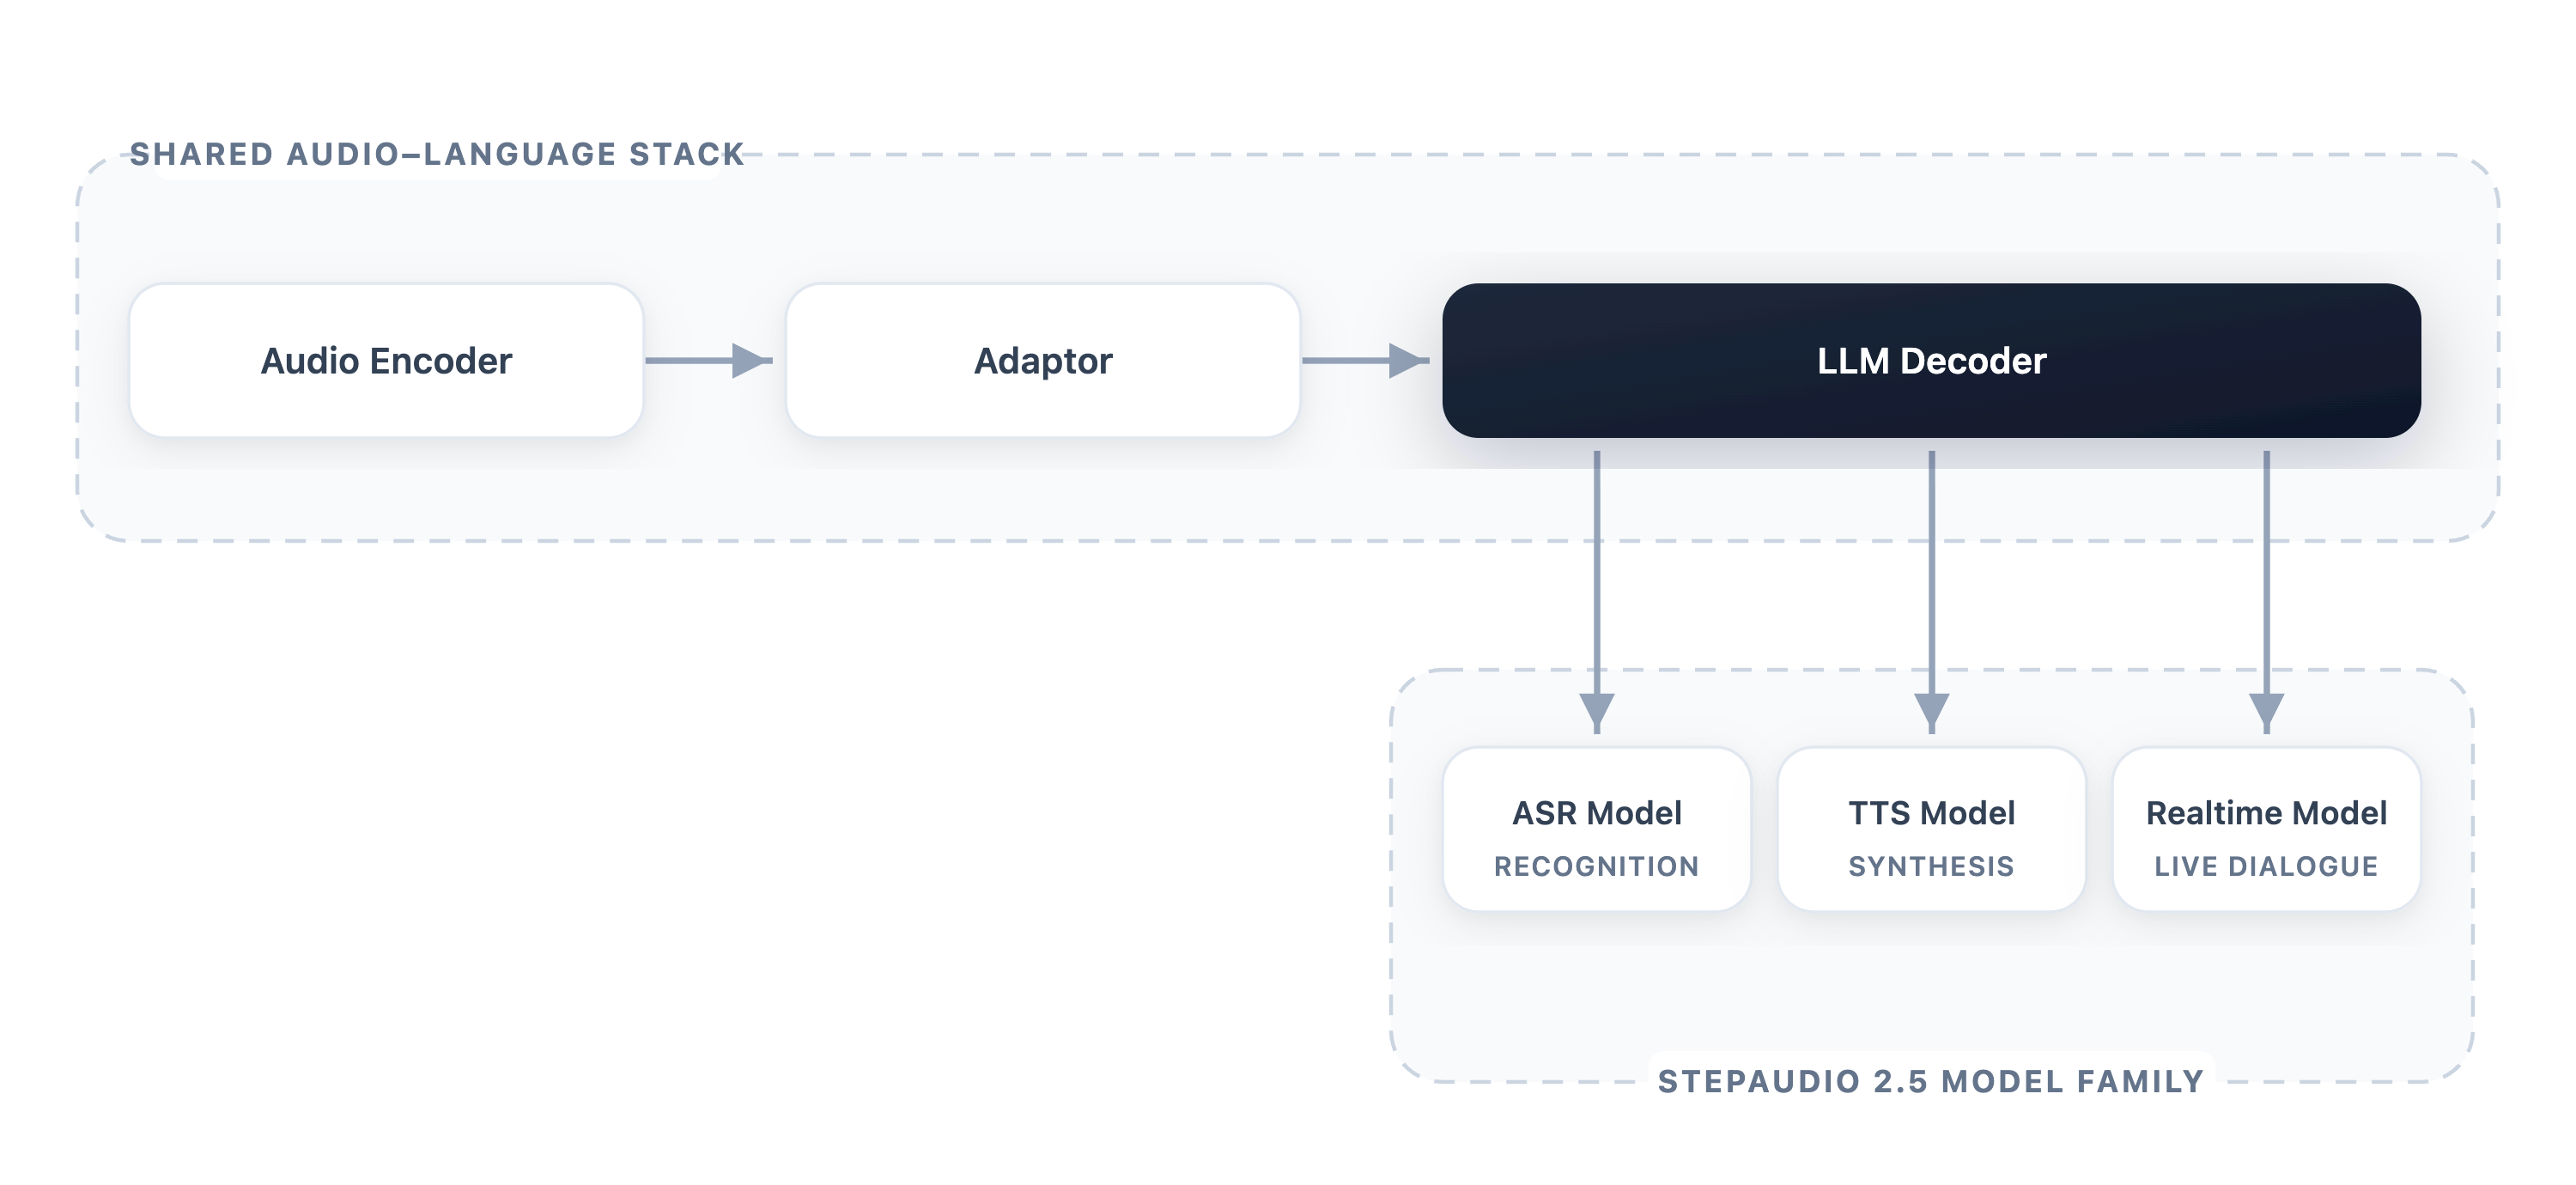
\includegraphics[width=1.0\linewidth]{figures/stepaudio25-unified-foundation-architecture.png}
\caption{A unified view of the StepAudio 2.5 model family. The shared audio-language stack provides the common architectural basis used to organize ASR, TTS, and Realtime, while the three systems serve different deployment goals.}
\label{fig:unified_architecture}
\end{figure}


\subsection{Task Specialization as Directional Inference}

StepAudio 2.5 supports three primary inference directions.
\begin{itemize}
\item In ASR, audio embeddings condition the decoder to generate transcript tokens. The output space is narrow, discrete, and strongly anchored by the speech signal.
\item In TTS, text and control instructions condition the decoder to generate audio tokens or intermediate audio representations. The output space is much richer, and the central challenge is not lexical correctness but faithful, natural, and expressive realization.
\item In Realtime, the model couples audio understanding and response generation under strict turn-level latency constraints, while maintaining conversational state, persona consistency, and contextual appropriateness.
\end{itemize}

This directional perspective provides a useful insight: the foundation model itself does not need separate notions of ``understanding'' and ``generation.'' It needs a single high-quality multimodal prior plus a mechanism to route supervision through different output spaces and deployment regimes. Recognition, synthesis, and realtime dialogue then become three ways of querying the same multimodal memory.
